\documentclass[12pt]{article}
 
\usepackage[margin=1in]{geometry}
\usepackage{amsmath,amsthm,amssymb, mathtools}
\usepackage[T1]{fontenc}
\usepackage{lmodern}
\usepackage{fixltx2e}
\usepackage[shortlabels]{enumitem}
\usepackage{mathrsfs}
\usepackage{kbordermatrix}

\usepackage{graphicx}

\renewcommand{\kbldelim}{(}% Left delimiter
\renewcommand{\kbrdelim}{)}% Right delimiter
 
\newcommand{\N}{\mathbb{N}}
\newcommand{\R}{\mathbb{R}}
\newcommand{\Z}{\mathbb{Z}}
\newcommand{\Q}{\mathbb{Q}}
 
\newenvironment{theorem}[2][Theorem]{\begin{trivlist}
\item[\hskip \labelsep {\bfseries #1}\hskip \labelsep {\bfseries #2.}]}{\end{trivlist}}
\newenvironment{lemma}[2][Lemma]{\begin{trivlist}
\item[\hskip \labelsep {\bfseries #1}\hskip \labelsep {\bfseries #2.}]}{\end{trivlist}}
\newenvironment{exercise}[2][Exercise]{\begin{trivlist}
\item[\hskip \labelsep {\bfseries #1}\hskip \labelsep {\bfseries #2.}]}{\end{trivlist}}
\newenvironment{problem}[2][Problem]{\begin{trivlist}
\item[\hskip \labelsep {\bfseries #1}\hskip \labelsep {\bfseries #2.}]}{\end{trivlist}}
\newenvironment{question}[2][Question]{\begin{trivlist}
\item[\hskip \labelsep {\bfseries #1}\hskip \labelsep {\bfseries #2.}]}{\end{trivlist}}
\newenvironment{corollary}[2][Corollary]{\begin{trivlist}
\item[\hskip \labelsep {\bfseries #1}\hskip \labelsep {\bfseries #2.}]}{\end{trivlist}}
\newcommand{\textfrac}[2]{\dfrac{\text{#1}}{\text{#2}}}
\newcommand{\floor}[1]{\left\lfloor #1 \right\rfloor}

\newenvironment{amatrix}[1]{%
  \left(\begin{array}{@{}*{#1}{c}|c@{}}
}{%
  \end{array}\right)
}

\DeclareMathOperator*{\E}{\mathbb{E}}


\begin{document}

\title{Stochastic Processes: Homework 2}

\author{Chris Hayduk}
\date{September 9, 2020}

\maketitle

\begin{problem}{1}
Durrett, Exercise 1.2
\end{problem}

Observe that if $0 < X_n < 5$, then there are 3 possibilities for the transition:
\begin{enumerate}
\item $X_{n+1} = X_n$. This can occur if two white balls are exchanged or if two black balls are exchanged
\item $X_{n+1} = X_n + 1$. This occurs if a black ball from the left urn is exchanged for a white ball from the right urn
\item $X_{n+1} = X_n - 1$. This occurs if a white ball from the left urn is exchanged for a black ball from the right urn
\end{enumerate}

If $X_n = 0$, then there is only one possible transition: $X_{n+1} = X_n + 1$.\\

If $X_n = 5$, then there is only one possible transition: $X_{n+1} = X_n - 1$.\\

From these facts, we can derive the transition probability matrix:
\begin{align*}
\kbordermatrix{
    & 0 & 1 & 2 & 3 & 4 & 5 \\
    0 & 0 & 1 & 0 & 0 & 0 & 0 \\
    1 & 0.04 & 0.32 & 0.64 & 0 & 0 & 0 \\
    2 & 0 & 0.16 & 0.48 & 0.36 & 0 & 0\\
    3 & 0 & 0 & 0.36 & 0.48 & 0.16 & 0 \\
    4 & 0 & 0 & 0 & 0.64 & 0.32 & 0.04\\
    5 & 0 & 0 & 0 & 0 & 1 & 0
  }
\end{align*}

Let $x = $ number of white balls in left urn and $y = $ number of white balls in right urn. Hence $5-x = $ number of black balls in left urn and $5-y = $ number of black balls in right urn.\\

Then for $0 < i < 5$, we have
\begin{align*}
p(i, i-1) &= \frac{x}{5} \cdot \frac{5-y}{5}\\
p(i, i) &= \frac{x}{5} \cdot \frac{y}{5} + \frac{5-x}{5} \cdot \frac{5-y}{5}\\
p(i, i+1) &= \frac{5-x}{5} \cdot \frac{y}{5}
\end{align*}

\newpage
\begin{problem}{2}
Durrett, Exercise 1.3
\end{problem}

Note that $X_n$ can be any integer from 0 to 5. Hence, the state space is $\{0, 1, 2, 3, 4, 5\}$.\\

For each individual roll $Y_k$, the possible sums are as follows, along with possible combinations to get that sum:
\begin{align*}
2:& (1, 1)\\
3:& (2, 1), (1, 2)\\
4:& (2, 2), (1, 3), (3, 1)\\
5:& (1, 4), (4, 1), (3, 2), (2, 3)\\
6:& (3, 3), (4, 2), (2, 4)\\
7:& (4, 3), (3, 4)\\
8:& (4, 4)
\end{align*}

We see that there are $16$ possible rolls with this pair of dice. Using the possible outcomes listed above, we can derive probabilities for each sum:
\begin{align*}
P(Y_k = 2) &= 0.0625\\
P(Y_k = 3) &= 0.125\\
P(Y_k = 4) &= 0.1875\\
P(Y_k = 5) &= 0.25\\
P(Y_k = 6) &= 0.1875\\
P(Y_k = 7) &= 0.125\\
P(Y_k = 8) &= 0.0625
\end{align*}

Now we can show which congruence classes these sums to modulo 6:
\begin{align*}
2 &= \bar{2}\\
3 &= \bar{3}\\
4 &= \bar{4}\\
5 &= \bar{5}\\
6 &= \bar{0}\\
7 &= \bar{1}\\
8 &= \bar{2}\\
\end{align*}

Now we can convert the probabilities for $Y_k$ using these congruence classes,
\begin{align*}
P(Y_k = \bar{0}) &= 0.1875\\
P(Y_k = \bar{1}) &= 0.125 + 0.125 = 0.25\\
P(Y_k = \bar{2}) &= 0.0625 + 0.0625 = 0.125\\
P(Y_k = \bar{3}) &= 0.125\\
P(Y_k = \bar{4}) &= 0.1875\\
P(Y_k = \bar{5}) &= 0.25\\
\end{align*}

Now using these probabilities and the properties of modular arithmetic, we will derive a transition probability matrix for $X_n$:
\begin{align*}
\kbordermatrix{
    & \bar{0} & \bar{1} & \bar{2} & \bar{3} & \bar{4} & \bar{5} \\
    \bar{0} & 0.1875 & 0.25 & 0.125 & 0.125 & 0.1875 & 0.25 \\
    \bar{1} & 0.25 & 0.1875 & 0.25 & 0.125 & 0.125 & 0.1875 \\
    \bar{2} & 0.1875 & 0.25 & 0.1875 & 0.25 & 0.125 & 0.125\\
    \bar{3} & 0.125 & 0.1875 & 0.25 & 0.1875 & 0.25 & 0.125 \\
    \bar{4} & 0.125 & 0.125 & 0.1875 & 0.25 & 0.1875 & 0.25\\
    \bar{5} & 0.25 & 0.125 & 0.125 & 0.1875 & 0.25 & 0.1875
  }
\end{align*}

So if $j \geq i$, we have 
\begin{align*}
p(i, j) = P(Y_{k} = \overline{j-i})
\end{align*}

\newpage
\begin{problem}{3}
Durrett, Exercise 1.58
\end{problem}

We have,
\begin{align*}
P(X_{n+1} = 1) - \frac{b}{a+b} &= P(X_{n+1} = 1 | X_n = 1)  \cdot P(X_n = 1) + P(X_{n+1} = 1 | X_n = 2) \cdot P(X_n = 2) - \frac{b}{a+b}\\
&= (1 - a)P(X_n = 1) + bP(X_n = 2) -  \frac{b}{a+b}\\
&= (1 - a)P(X_n = 1) + b(1 - P(X_n = 1)) -  \frac{b}{a+b}\\
&= (1 - a - b)P(X_n = 1) + b -  \frac{b}{a+b}\\
&= (1 - a - b)P(X_n = 1) + \frac{b(a+b)}{a+b} -  \frac{b}{a+b}\\
&= (1 - a - b)P(X_n = 1) + \frac{b(a+b) - b}{a+b}\\
&= (1 - a - b)P(X_n = 1) + \frac{b(a + b - 1)}{a+b}\\
&= (1 - a - b)P(X_n = 1) - \frac{b(1 - a - b)}{a+b}\\
&= (1 - a - b) \left[P(X_n = 1) - \frac{b}{a+b}\right]
\end{align*}

Note that,
\begin{align*}
P(X_n = 1) - \frac{b}{a+b} &= (1 - a - b) \left[P(X_{n-1} = 1) - \frac{b}{a+b}\right]\\
&= (1 - a - b) \left[(1-a-b)\left(P(X_{n-2} = 1) - \frac{b}{a+b}\right)\right]\\
&= (1 - a - b)^2 \left[P(X_{n-2} = 1) - \frac{b}{a+b}\right]\\
&= (1 - a - b)^3 \left[P(X_{n-3} = 1) - \frac{b}{a+b}\right]\\
&\vdots\\
&= (1 - a - b)^n \left[P(X_{0} = 1) - \frac{b}{a+b}\right]
\end{align*}

So this gives us,
\begin{align*}
P(X_n = 1) &= \frac{b}{a+b} + (1 - a - b)^n \left[P(X_{0} = 1) - \frac{b}{a+b}\right]
\end{align*}

\newpage
\begin{problem}{4}
\end{problem}

\begin{enumerate}[label=(\Alph*)]

\item We consider the following matrix,
\begin{align*}
p = \kbordermatrix{
    & 1 & 2 & 3 \\
    1 & 0 & 1 & 0\\
    2 & 0 & 1/2 & 1/2\\
    3 & 1/2 & 0 & 1/2
  }
\end{align*}

Now we take $p - \lambda I$
\begin{align*}
p - \lambda I &= \kbordermatrix{
    & 1 & 2 & 3 \\
    1 & 0 & 1 & 0\\
    2 & 0 & 1/2 & 1/2\\
    3 & 1/2 & 0 & 1/2
  } - \kbordermatrix{
    & 1 & 2 & 3 \\
    1 & \lambda & 0 & 0\\
    2 & 0 & \lambda & 0\\
    3 & 0 & 0 & \lambda
  }\\
&= \kbordermatrix{
    & 1 & 2 & 3 \\
    1 & -\lambda & 1 & 0\\
    2 & 0 & 1/2 - \lambda & 1/2\\
    3 & 1/2 & 0 & 1/2 - \lambda
  }
\end{align*}

Now we need to find $det(p - \lambda I)$,
\begin{align*}
det(p - \lambda I) &= -\lambda \begin{vmatrix}
1/2 - \lambda & 1/2\\
0 & 1/2 - \lambda
\end{vmatrix} - 1 \begin{vmatrix}
0 & 1/2\\
1/2 & 1/2 - \lambda
\end{vmatrix} + 0 \begin{vmatrix}
0 & 1/2 - \lambda\\
1/2 & 0
\end{vmatrix}\\
&= -\lambda \begin{vmatrix}
1/2 - \lambda & 1/2\\
0 & 1/2 - \lambda
\end{vmatrix} - \begin{vmatrix}
0 & 1/2\\
1/2 & 1/2 - \lambda
\end{vmatrix}\\
&= -\lambda[(1/2-\lambda)^2 - 0] - (0 - 1/4)\\
&= -\lambda(\lambda^2 - \lambda + 1/4) + 1/4\\
&= -\lambda^3 + \lambda^2 - \lambda/4 + 1/4
\end{align*}

Lastly, we need to solve
\begin{align*}
-\lambda^3 + \lambda^2 - \lambda/4 + 1/4 = 0
\end{align*}

The solutions to this equation are:
\begin{align*}
\lambda_1 &= 1\\
\lambda_2 &= -i/2\\
\lambda_3 &= i/2
\end{align*}

\newpage
\item By diagonalization, we have that,
\begin{align*}
p &= X\Lambda X^{-1}\\
p^2 &= X\Lambda X^{-1} X\Lambda X^{-1} = X\Lambda^2 X^{-1}\\
&\vdots\\
p^n &= X\Lambda^n X^{-1}
\end{align*}

where $X$ is the matrix whose columns are the eigenvectors of $p$ and $\Lambda$ is the matrix with the eigenvalues of $p$ on the diagonal and $0$s everywhere else.\\

Now to find the three eigenvectors:
\begin{align*}
(p - \lambda_1 I)x_1 &= 0\\
(p - \lambda_2 I)x_2 &= 0\\
(p - \lambda_3 I)x_3 &= 0
\end{align*}

The solutions to these equations are:
\begin{align*}
x_1 &= (1, 1, 1)\\
x_2 &= (-1 - i, -\frac{1}{2} + \frac{i}{2}, 1)\\
x_3 &= (-1 + i, -\frac{1}{2} - \frac{i}{2}, 1)
\end{align*}

So,
\begin{align*}
X &= \begin{bmatrix}
1 & -1 - i & -1 + i\\
1 & -\frac{1}{2} + \frac{i}{2} & -\frac{1}{2} - \frac{i}{2}\\
1 & 1 & 1
\end{bmatrix}
\end{align*}

and the inverse is,
\begin{align*}
X^{-1} &= \begin{bmatrix}
\frac{1}{5} & \frac{2}{5} & \frac{2}{5}\\
-\frac{1}{10} + \frac{3i}{10} & -\frac{1}{5} - \frac{2i}{5} & \frac{3}{10} + \frac{i}{10}\\
-\frac{1}{10} - \frac{3i}{10} & -\frac{1}{5} + \frac{2i}{5} & \frac{3}{10} - \frac{i}{10}
\end{bmatrix}
\end{align*}

Lastly, we have
\begin{align*}
\Lambda^n &= \begin{bmatrix}
1 & 0 & 0\\
0 & -\frac{i}{2} & 0\\
0 & 0 & \frac{i}{2}
\end{bmatrix}^n\\
&= \begin{bmatrix}
1 & 0 & 0\\
0 & -\frac{i}{2}^n & 0\\
0 & 0 & \frac{i}{2}^n
\end{bmatrix}
\end{align*}
So we have,
\begin{align*}
p^n &= X \Lambda^n X^-1
\end{align*}

which yields

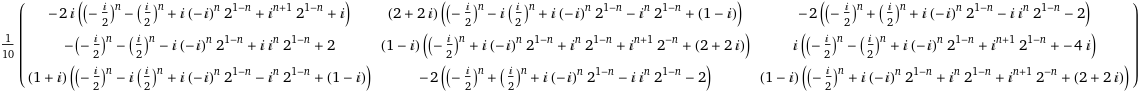
\includegraphics[scale=0.42]{matrix.png}

Hence,
\begin{align*}
p^n(1,1) &= -\frac{2i}{10}\left(\left(-\frac{i}{2}\right)^n - \left(\frac{i}{2}\right)^n + i(-i)^n2^{1-n} + i^{n+1}2^{1-n} + i\right)\\
&=  -\frac{2i}{10}\left(-\frac{i}{2}\right)^n -  -\frac{2i}{10}\left(\frac{i}{2}\right)^n + \frac{2^{1-n+1}(-i)^n}{10} - \frac{2^{1-n+1}i^{n+2}}{10} + i\\
&= -\frac{2i}{10}\left(-\frac{i}{2}\right)^n -  -\frac{2i}{10}\left(\frac{i}{2}\right)^n + \frac{2^{1-n+1}((-i)^n - i^{n+2})}{10} + i\\
&= -\frac{2i}{10}\left(-\frac{i}{2}\right)^n -  -\frac{2i}{10}\left(\frac{i}{2}\right)^n + 1^n\left(\frac{2^{1-n+1}((-i)^n - i^{n+2})}{10} + i\right)\\
&= -\frac{2i}{10}\left(-\frac{i}{2}\right)^n -  -\frac{2i}{10}\left(\frac{i}{2}\right)^n + 1^n\left(\frac{2^{1-n+1}((-i)^n - i^{n+2})}{10} + i\right)\\
&= \left(\frac{2^{1-n+1}((-i)^n - i^{n+2})}{10} + i\right)\lambda_1^n -\frac{2i}{10}\lambda_2^n -  -\frac{2i}{10}\lambda_3^n\\
&= \left(\frac{2^{1-n}((-i)^n - i^{n+2})}{5} + i\right)\lambda_1^n -\frac{i}{5}\lambda_2^n -  -\frac{i}{5}\lambda_3^n\\
&= \left(\frac{2^{1-n}((-1)^n(i^n - i^{n+2}))}{5} + i\right)\lambda_1^n -\frac{i}{5}\lambda_2^n -  -\frac{i}{5}\lambda_3^n\\
&=\left(\frac{2^{1-n}(-1)^n(1-i^2)i^n}{5} + i\right)\lambda_1^n -\frac{i}{5}\lambda_2^n -  -\frac{i}{5}\lambda_3^n\\
&=\left(\frac{2^{1-n}(-1)^n2i^n}{5} + i\right)\lambda_1^n -\frac{i}{5}\lambda_2^n -  -\frac{i}{5}\lambda_3^n\\
&=\left(\frac{2^{1-n+1}(-1)^ni^n}{5} + i\right)\lambda_1^n -\frac{i}{5}\lambda_2^n -  -\frac{i}{5}\lambda_3^n
\end{align*}

as required. 

\newpage
\item We have the following equations:
\begin{align*}
p^0(1, 1) &= 1 = a + b + c\\
p^1(1, 1) &= 0 = a\lambda_1 + b\lambda_2 + c\lambda_3 = a +\frac{-i}{2}b + \frac{i}{2}c\\
p^2(1, 1) &= 0 = a\lambda_1^2 + b\lambda_2^2 + c\lambda_3^2 = a + \frac{-1}{4}b + \frac{-1}{4}c
\end{align*}

We can set up an augmented matrix for this system of equations:
\begin{align*}
\begin{amatrix}{3}
1 & 1 & 1 & 1\\
1 & \frac{-i}{2} & \frac{i}{2} & 0\\
1 & \frac{-1}{4} & \frac{-1}{4} & 0
\end{amatrix}
\end{align*}

Row reduction yields:
\begin{align*}
\begin{amatrix}{3}
1 & 0 & 0 & \frac{1}{5}\\
0 & 1 & 0 & \frac{2}{5} - \frac{i}{5}\\
0 & 0 & 1 & \frac{2}{5} + \frac{i}{5}
\end{amatrix}
\end{align*}

Hence we have,
\begin{align*}
p^n(1, 1) &= \frac{1}{5} + \left(\frac{2}{5} - \frac{i}{5}\right) \cdot \frac{-i}{2}^n + \left(\frac{2}{5} + \frac{i}{5}\right) \cdot \frac{i}{2}^n
\end{align*}

\item If $n$ even:
\begin{align*}
p^n(1, 1) &= \frac{1}{5} + \left(\frac{2}{5} - \frac{i}{5}\right) \cdot \frac{-1}{2^n} + \left(\frac{2}{5} + \frac{i}{5}\right) \cdot \frac{-1}{2^n}\\
&= \frac{1}{5} + \frac{-2}{5 \cdot 2^n} - \frac{-i}{5 \cdot 2^n} + \frac{-2}{5 \cdot 2^n} + \frac{-i}{5 \cdot 2^n}\\
&= \frac{1}{5} + \frac{-4}{5 \cdot 2^n}
\end{align*}

If $n$ odd:
\begin{align*}
p^n(1, 1) &= \frac{1}{5} + \left(\frac{2}{5} - \frac{i}{5}\right) \cdot \frac{-i}{2^n} + \left(\frac{2}{5} + \frac{i}{5}\right) \cdot \frac{i}{2^n}\\
&= \frac{1}{5} + \frac{-2i}{5 \cdot 2^n} - \frac{1}{5 \cdot 2^n} + \frac{2i}{5 \cdot 2^n} + \frac{-1}{5 \cdot 2^n}\\
&= \frac{1}{5} + \frac{-2}{5 \cdot 2^n}
\end{align*}

In either case, we see that as $n \to \infty$, the second term goes to $0$. Hence, we have that,
\begin{align*}
p^n(1, 1) \to \frac{1}{5} \; \text{as} \; n \to \infty
\end{align*}

\end{enumerate}
\end{document}